\documentclass[12pt,a4paper]{report}
\usepackage[utf8]{inputenc}
\usepackage{amsmath}
\usepackage{amsfonts}
\usepackage{amssymb}
\usepackage{graphicx}
\usepackage{lmodern}
\usepackage[left=2cm,right=2cm,top=2cm,bottom=2cm]{geometry}
%%%%%%%%%%%%%%%%%%
% Set color
\usepackage[dvipsnames]{xcolor}
\usepackage{sectsty}
\chapterfont{\color{MidnightBlue}}  % sets colour of chapters
\sectionfont{\color{MidnightBlue}}
\subsectionfont{\color{MidnightBlue}}

%%%%%%%%%%%%%%%%%%%%%%%%
% Itemize Color
\usepackage{enumitem}
\newlist{mylist1}{itemize}{1}
\setlist[mylist1]{label={\textcolor{red}{\begin{math}
    \blacksquare
\end{math}}}}

\newlist{mylist2}{itemize}{2}
\setlist[mylist2]{label={\textcolor{MidnightBlue}{\begin{math}
    \blacktriangleright
\end{math}}}}
%%%%%%%%%%%%%%%%%%%%%%%%%%%%%%%%%%%%
%Tabel of contents
\usepackage{hyperref}
\hypersetup{
    colorlinks,
    citecolor=black,
    filecolor=black,
    linkcolor=black,
    urlcolor=green
}

%%%%%%%%%%%%%%%%%%%%%%%%%%%%%%%%%%%%%%%%%%
\begin{document}
\title{\textcolor{MidnightBlue}{\textbf{\Huge Azure Fundamentals (AZ - 900)}}}
\author{\Large Manjunath Prasad Holenarasipura Rajiv}
\maketitle
\tableofcontents
\clearpage
\chapter{Describe Cloud Concepts}
\section{Describe Cloud Computing}
\subsection{Introduction to Cloud Computing}
\begin{mylist1}
    \item Cloud Computing is a delivery of computing services
    over the internet
\end{mylist1}
\subsection{Shared Responsibility Model}
\begin{mylist1}
    \item Cloud Provider Responsibility
    \begin{mylist2}
        \item Physical Security
        \item Power
        \item Cooling
        \item Network Connectivity
    \end{mylist2}
    \item Consumer Responsibility
    \begin{mylist2}
        \item Data and Information stored in the cloud
        \item Devices
        \item Acccounts and Identities
        \item Access Security $-$ Give access to those who need it
    \end{mylist2}
\end{mylist1}

\subsection{Cloud Models}
\begin{mylist1}
    \item Private Cloud
    \begin{mylist2}
        \item Used by single entity
        \item Provides more control
        \item Greater cost and fewer benefits of public Cloud
        \item It can be hosted from onsite or offsite data center
    \end{mylist2}
    \item Public Cloud
    \begin{mylist2}
        \item Built, controlled and maintained by third party cloud Provider
        \item Purchase and access cloud resources
    \end{mylist2}
    \item Hybrid Cloud
    \begin{mylist2}
        \item Uses both private and public clouds in an inter $-$ connected environment
        \item Allow a private cloud to surge for increased, temporary demand by deploying public cloud resources  
        \begin{figure}[!htpb]
            \centering
            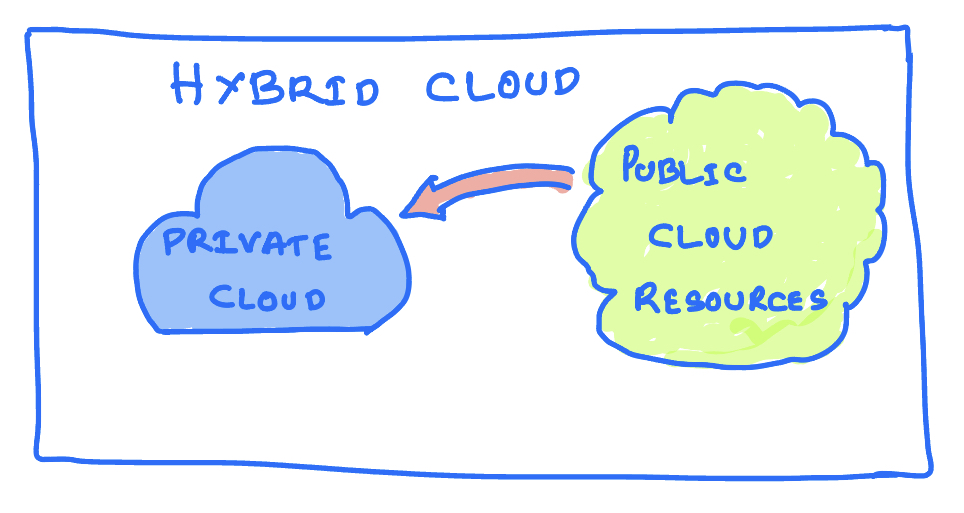
\includegraphics[scale=0.20]{/LaTeX/Notes Templates/Document/Images/hybrid.jpg}
        \end{figure}
    \end{mylist2}
    \item Multi Cloud
    \begin{mylist2}
        \item Multiple cloud providers are used.
    \end{mylist2}
    \item Azure Arc
    \begin{mylist2}
        \item Azure arc is a set of technologies helps to mange cloud environment.
    \end{mylist2}
\end{mylist1}
\subsection{Consumption-based Model}
\begin{mylist1}
\item Types of Expenses
\begin{mylist2}
    \item Capital Expense (CapEx) is one-time up-front expenditure to purchase resources.
    \item Operation Expense (OpEx) is spending over time for resources. Cloud Computing is OpEx and pay-as-you-go model.
\end{mylist2}
\end{mylist1}
\section{Describe Benefits of Cloud Computing}
\subsection{Describe the benefits of Availability and Scalability in the cloud}
\begin{mylist1}
    \item High Availability
    \begin{mylist2}
        \item High availability focuses on ensuring maximum availability, regardless of disruptions or events that may occur.
    \end{mylist2}
    \item Scalability
    \begin{mylist2}
        \item Scalability refers to the ability to adjust resources to meet demand.
        The ability to scale means you can add more resources to better handle the increased demand.
        \item \textbf{Vertical Scalability} $-$ With vertical scaling, if you were developing an app and you needed more processing power, you could vertically scale up to add more CPUs or RAM to the virtual machine. Conversely, if you realized you had over-specified the needs, you could vertically scale down by lowering the CPU or RAM specifications.
        \item \textbf{Horizontal Scalability} $-$ With horizontal scaling, if you suddenly experienced a steep jump in demand, your deployed resources could be scaled out. 
    \end{mylist2}
\end{mylist1}
\subsection{Describe the benefits of reliability and predictability in the cloud}
\begin{mylist1}
    \item Reliability
    \begin{mylist2}
        \item Reliability is the ability of a system to recover from failures and continue to function.
    \end{mylist2}
    \item Predictability
    \begin{mylist2}
        \item Predictability can be focused on performance predictability or cost predictability
        \item Cost predictability is focused on predicting or forecasting the cost of the cloud spend. 
        \item Performance predictability focuses on predicting the resources needed to deliver a positive experience for your customers.
    \end{mylist2}
\end{mylist1}
\subsection{Describe the benefits of security and governance in the cloud}
\begin{mylist1}
    \item Security $-$ Find a cloud solution that matches your security needs.
    \item Governance $-$ By establishing a good governance footprint early, you can keep your cloud footprint updated, secure, and well managed.
\end{mylist1}
\subsection{Describe the benefits of manageability in the cloud}
\begin{mylist1}
    \item Management of the cloud
    \begin{mylist2}
        \item Automatically scale resource deployment based on need.
        \item Deploy resources based on a preconfigured template, removing the need for manual configuration.
        \item Monitor the health of resources and automatically replace failing resources.
        \item Receive automatic alerts based on configured metrics, so you’re aware of performance in real time.
    \end{mylist2}
    \item Management in the cloud
    \begin{mylist2}
        \item Through a web portal.
        \item Using a command line interface.
        \item Using APIs.
        \item Using PowerShell.
    \end{mylist2}
\end{mylist1}
\section{Describe cloud service types}
\subsection{Describe Infrastructure as a Service}
\begin{mylist1}
    \item Provides you the maximum amount of control for your cloud resources
    \item The cloud provider is responsible for maintaining the physical infrastructure and its access to the internet. You’re responsible for installation and configuration, patching and updates, and security.
    \item Scenarios
    \begin{mylist2}
        \item Lift-and-shift migration: You’re standing up cloud resources similar to your on-prem datacenter, and then simply moving the things running on-prem to running on the IaaS infrastructure.
        \item Testing and development: You have established configurations for development and test environments that you need to rapidly replicate. You can stand up or shut down the different environments rapidly with an IaaS structure, while maintaining complete control.
    \end{mylist2}
\end{mylist1}

\subsection{Describe Platform as a Service}
\begin{mylist1}
    \item In a PaaS environment, the cloud provider maintains the physical infrastructure, physical security, and connection to the internet.
    \item They also maintain the operating systems, middleware, development tools, and business intelligence services that make up a cloud solution.
    \item The cloud provider is responsible for maintaining the physical infrastructure and its access to the internet, just like in IaaS.
    \item In the PaaS model, the cloud provider will also maintain the operating systems, databases, and development tools.
    \item Scenarios
    \begin{mylist2}
        \item Development framework: PaaS provides a framework that developers can build upon to develop or customize cloud-based applications.
        \item Analytics or business intelligence: Tools provided as a service with PaaS allow organizations to analyze and mine their data, finding insights and patterns and predicting outcomes to improve forecasting, product design decisions, investment returns, and other business decisions.
    \end{mylist2}
\end{mylist1}

\subsection{Describe Software as a Service}
\begin{mylist1}
    \item Software as a service (SaaS) is the most complete cloud service model from a product perspective.
    \item SaaS is the model that places the most responsibility with the cloud provider and the least responsibility with the user.
    \item In a SaaS environment you're responsible for the data that you put into the system, the devices that you allow to connect to the system, and the users that have access. Nearly everything else falls to the cloud provider.
    \item The cloud provider is responsible for physical security of the datacenters, power, network connectivity, and application development and patching.
    \item Scenarios
    \begin{mylist2}
        \item Email and messaging.
        \item Business productivity applications.
        \item Finance and expense tracking.
    \end{mylist2}
\end{mylist1}
\chapter{Describe Azure Architecture and Services}
\section{}
\chapter{Describe Azure Management and Governance}
\section{}

\begin{mylist2}
    \item 
    \item 
\end{mylist2}

\end{document}